\documentclass{article}
\usepackage{graphicx}


\begin{document}
\title{Technical Document}
\date{\today}
\author{Kyle Chuang, Josh Wilson, Jessica Economou}
%  \maketitlepage

%  \newpage
\section{General Overview}

 There is an extensive literature in traffic management on how to identify and to quantify hotspots, which are locations that are particularly dense with accidents or with fatalities. Our proposed hotspot analysis employs a novel algorithm, HDBScan, to the FARS data set. This is the first documented implementation of HDBScan to the hotspot problem and is consequently different from some of the more commonly accepted measures of fatalizes/mile across roadways. Fatalities/mile, for example, struggles to account for the features (e.g. time, presence of alcohol, demographic variables of drivers) of the crash, because it only considers the density of the occurrences on a stretch of road. On the other hand, the HDBScan algorithm has been designed to incorporate a host of features when creating its clusters. As a result, the user is able to devote more time to focus on identifying the leading factors associated with fatal accidents, which could lead to benefits in deploying solutions to those areas.

Further difficulties in hotspot detection stem from year-over-year variability in traffic patterns and subsequent distributions of accidents. It has been noted that hotspots may disappear and reappear, when looking at data on a year over year basis. For example, an algorithm could decide that a certain area is a hotspot on odd numbered years and not on even numbered years. This complexity in determining persistent clusters can be an acute challenge for traffic engineers and for policy experts who advise committees on budget allocation.

\section{Clustering Algorithm Selection}
Unsupervised learning and data mining efforts have produced numerous types of clustering algorithms. The most popularly applied algorithms include K-Nearest Neighbors (KNN), K-Means, and Gaussian Mixture Models (GMM). Unfortunately, those popular algorithms were not suitable for the problem posed, because they group instances based on similarity within the cluster. For KNN/K-means, the weakness stems from stability. Multiple runs are typically required to assess stability and there are no guarantees of stability within each run for any given data point. For GMM and K-means, the spherical/elliptical constraints for each cluster may not be appropriate for a traffic analysis problem as hotspots may run along an unconstrained road or a geographic feature. Finally, the clustering algorithms provided above are unable to classify points as "not in cluster". Even with modified methods of "cutting" off points at a given distance/probability (K-mean/GMM) as unclustered, other weaknesses make the algorithms provided inapproriate for geostatistical analyses.

\section{HDBScan}
HDBScan (hierarchical density based scan) was chosen as the clustering algorithm. HDBScan is a clustering algorithm based on density. It is non-parametric and shapewise unconstrained. The algorithm is also consistent and stable. Repeated runs of the algorithm will always provide the same results unlike some of the algorithms mentioned above. Additionally, it can classify data points as not in any cluster based on cluster stability and density.  HDBScan can succintly be described as clustering based on how close the data points are relative to each other in a given area.


HDBScan begins by taking $n$ samples closest points for each data point. The $n$ sample circlular space radius is called the core distance. After the core distances has been determined, the algorithm computes the reachability for all data points. Reachability is defined as the maximum distance between the 2 point or core distance. A hierachical tree is built based on reachability metric. Clusters are determined based on stability of the parent tree structure compared to the children node tree structurei.\footnote{For a more detailed discussion, please refer to the following link -  https://hdbscan.readthedocs.io/en/latest/how\_hdbscan\_works.html.}

\section{Methodology}
The clustering methodology based on HDBScan can be described as follows:
\begin{enumerate}
	\item Perform the clustering for each year from the algorithm below (yearly clustering algorithm).
	\begin{enumerate}
			\item Select all the points where the variable of interest is active and drop all the other points. For example, select all data points where the accident involved a rollover and drop all the other data points.
			\item Cluster the selected points based on geographic location using the manhattan distance metric.
			\item Create a polygon (convex hull) from each clusters found to determine the problem area.
			\item Label all data points to belong to cluster $x$ if they are inside the boundaries of polygon $x$.
			\item Perform a significance test for all point inside a cluster polygon against all unclustered points. A $p-value$ of 0.05 is determined to be significant. If a cluster is not found to be significant, it is relabeled as unclustered.\footnote{The significance test used was the wilcoxon ranked sum test. This was chosen over t-test since it was non-parametric. To satisfy the normality constraint of the t-test, hundreds of data points were required. The number of data points and normality was empirically determined using sampling and the shapiro-wilks normality test. The $\chi^2$-test was not chosen since the data was not always symmetric.}
	\end{enumerate}
	\item Once all years has been clustered, overlay the cluster polygons on top of each other geographically. Find the intersections of all polygons that overlap more than $n$ years. The intersections are now time-based cluster polygons.
	\item Relabel all points based on time-based cluster polygons for cluster determination.\footnote{The time-based cluster polygons were expanded by 0.01\% (approximately 1/2 mile in distance) to ensure the inclusion of the polygon vertices itself. The alternative was to iterate through the entire dataset and check for the points on the vertices/edges. This was done to improve the computational speed for efficient visualization.}
	\item Perform a significance test for all points inside time-based cluster polygons against all unclusterd points. If time-based cluster polygon is not found to be significant, the points are relabeled as unclustered.
\end{enumerate}
From a statistical perspective, the yearly clustering algorithm should identify a false positive cluster only 1 out of 20 times if random points from that particular year's dataset to form a a cluster. The false positive cluster rate for time-based polygon clusters will be the same assuming random points are selected from all available years.

An example is provided below using an intersection of 2 years. Each colored polygon is a significant cluster polygon for each individual year. However, only the red colored data points are significant clusters across time. Note that the red data points include both rollovers and non-rollover fatalities. The areas with the group of red data points, however, has a statistically siginficant different mean from all other areas in the state.
\begin{center}
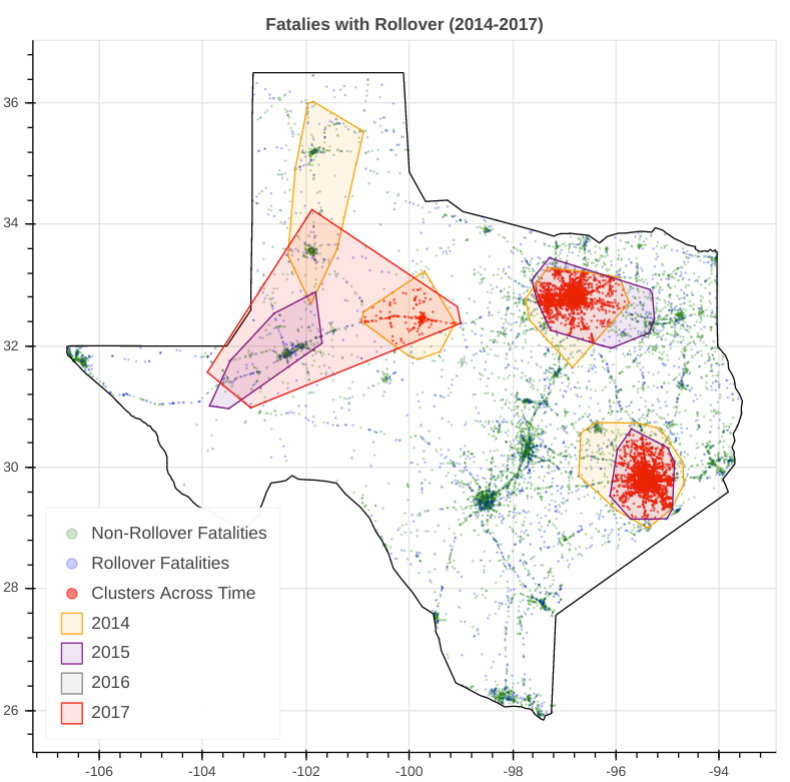
\includegraphics[scale=0.4]{technical.png}
\end{center}
From the map above, there appears to be cluster in a rural flat area in West Texas. The West Texas area is extremely flat and low desnity, the cluster appearance is unexpected. Since rollovers are likely to require high speeds in flat areas, a hypothesis of excessive speeding in the area may be further examined. This can easily be contrasted with Austin area, which is hilly, higher density and does not have any rollover clusters.

\end{document}
